\ifx\XeTeXversion\undefined\pdfoutput=1\fi
\documentclass[11pt,reqno]{amsart}

\usepackage[margin=0.98in]{geometry}
\usepackage{amsmath,amssymb,amsthm,mathtools}
\usepackage{booktabs,array,multirow}
\usepackage{graphicx}
\usepackage{xcolor}
\usepackage{enumitem}
\usepackage{microtype}
\usepackage{listings}
% Allow line breaks after underscores inside long identifiers
\let\origunderscore\_
\renewcommand{\_}{\origunderscore\allowbreak}
\setlength{\emergencystretch}{3em}
\allowdisplaybreaks[1]
\usepackage[colorlinks=true,linkcolor=blue!60!black,citecolor=teal!70!black,urlcolor=blue!70!black]{hyperref}
\pdfstringdefDisableCommands{\let\_\origunderscore}
\renewcommand{\paragraph}[1]{\medskip\noindent\textbf{#1}\enspace}

% Theorem environments
\newtheorem{theorem}{Theorem}[section]
\newtheorem{proposition}[theorem]{Proposition}
\newtheorem{lemma}[theorem]{Lemma}
\newtheorem{corollary}[theorem]{Corollary}
\theoremstyle{definition}
\newtheorem{definition}[theorem]{Definition}
\newtheorem{remark}[theorem]{Remark}

% Clean code listings (pure ASCII safe for arXiv pdflatex)
\lstdefinelanguage{Lean4}{
  keywords={abbrev,def,noncomputable,theorem,lemma,structure,inductive,where,if,then,else,fun,by,in,forall,exists,Set,Fin,Real,Int,Nat,Array,List},
  sensitive=true,
  morecomment=[l]{--},
  morecomment=[s]{/-}{-/}
}
\lstset{
  language=Lean4,
  basicstyle=\ttfamily\footnotesize,
  keywordstyle=\bfseries\color{blue!60!black},
  commentstyle=\itshape\color{black!55},
  frame=single,
  framerule=0.4pt,
  rulecolor=\color{black!25},
  backgroundcolor=\color{black!2},
  xleftmargin=0.8em,
  xrightmargin=0.8em,
  aboveskip=0.8em,
  belowskip=0.8em,
  breaklines=true,
  columns=fullflexible
}

% Standard notation
\newcommand{\R}{\mathbb{R}}
\newcommand{\C}{\mathbb{C}}
\newcommand{\Q}{\mathbb{Q}}
\newcommand{\Z}{\mathbb{Z}}
\newcommand{\N}{\mathbb{N}}
\newcommand{\Sph}{\mathbb{S}^2}
\newcommand{\ip}[2]{\langle #1, #2 \rangle}
\newcommand{\norm}[1]{\lVert #1 \rVert}
\newcommand{\Xstar}{X^*_{11}}
\newcommand{\Elb}{E_{\mathrm{lb}}}
\newcommand{\Eub}{E_{\mathrm{ub}}}

\title[Certified Bounds and Three-Point Obstruction for Thomson \texorpdfstring{$N = 11$}{N = 11}]{%
Certified Two-Sided Energy Bounds in Lean~4 and the Three-Point Semidefinite Obstruction for the Eleven-Point Thomson Problem}

\author{Yang Li}
\address{Changsha University of Science and Technology, Changsha, China}
\email{ly3069777195@outlook.com}

\subjclass[2020]{Primary 52A40, 31C20; Secondary 90C22, 68V20, 52C17}
\keywords{Thomson problem, Coulomb energy, spherical codes, three-point semidefinite programming bounds, four-point semidefinite hierarchy, Lean~4, computer-assisted proof}

\date{November 24, 2026}

\begin{document}

\begin{abstract}
We investigate the eleven-point Thomson problem of minimizing the discrete Coulomb energy
\[
  E(x) \;=\; \sum_{0 \le i < j < 11} \frac{1}{\norm{x_i - x_j}}
\]
over configurations of eleven distinct points on the unit sphere $\Sph \subset \R^3$.
First, we establish a fully kernel-checked two-sided rational energy bracket in Lean~4 over Mathlib (\texttt{leanprover/lean4:v4.34.1}):
\[
  40.55547170437074 = \frac{2027773585218537}{50000000000000}
  \le E_1(11) \le
  \frac{2029822525409531}{50000000000000} = 40.59645050819062,
\]
together with formal proofs of the elementary milestones $E(x) \ge 55/2$ and $E(x) \ge 155/4$.
The lower bound is certified via an $S_3$-equivariant degree-$18$ three-point semidefinite programming (SDP) certificate at order $(M,K) = (10,10)$, verified inside the Lean~4 kernel through a zero-Mathlib \texttt{Init} data layer, binary bit-tries, and $19$ parallel two-dimensional Kronecker evaluation slices.
The upper bound is realized by an explicit rational $C_{2v}$ configuration constructed via north-pole stereographic projection (stored as pure integer Pythagorean quadruples with zero square roots), lying within $1.46 \times 10^{-14}$ of the $80$-digit stationary energy $E^*(11) \approx 40.59645050819060538664$.
All Lean proofs use zero \texttt{sorry}s, no \texttt{native\_decide}, and only Lean's three standard axioms (\texttt{propext}, \texttt{Classical.choice}, \texttt{Quot.sound}).

Second, we explain why the remaining gap $\Delta \approx 0.0410$ does not close under the three-point SDP framework that recently settled $N = 7, 8, 9$.
Using $15$ independently verified exact rational certificates ($410$ positive-definite blocks) extending up to degree $22$ at $(M,K)=(12,12)$ ($E_{\mathrm{cert}} = 40.556960329409$, $\Delta = 0.039490$), cap truncations, and $(2,9)$-typed pole-ring strips, we diagnose an intrinsic \emph{fractional-icosahedral pseudo-moment obstruction}: the optimal dual three-point pseudo-measure places $3.395$ fractional antipodal pairs near $t = -1$ and exhibits the exact icosahedral $I_h$ harmonic parity selection rule ($F_9, F_{11}$ inactive, $F_{10}$ active), bypassing the $\R^3$ four-point rank-$3$ determinant constraint $\det G_4 = 0$ that imposes a sharp energy wall on true spherical configurations with $k \ge 3$ antipodal pairs.
Finally, we implement an exact rational $S_{11} \times O(3)$-reduced coupled four-point SDP hierarchy probe, proving strict matched-degree lifts ($+0.1631$ at degree~$6$, $+0.00782$ at degree~$8$) while demonstrating that breaking the $\approx 40.557$ three-point ceiling requires four-point degree $D_4 \ge 14$ or multi-pair matching branch-and-bound.
\end{abstract}

\maketitle

\section{Introduction}\label{sec:intro}

Given $N$ distinct points $x = (x_0,\dots,x_{N-1})$ on the unit sphere $\Sph = \{v \in \R^3 : \norm{v} = 1\}$, the \emph{Thomson problem}~\cite{Thomson1904} asks for the global minimum
\begin{equation}\label{eq:energy}
  E_1(N) \;:=\; \inf_{x \in \mathrm{SphereConfig}(N)} E(x),
  \qquad E(x) \;=\; \sum_{0 \le i < j < N} \frac{1}{\norm{x_i - x_j}} \;=\; \sum_{0 \le i < j < N} \varphi(\ip{x_i}{x_j}),
\end{equation}
where $\varphi(t) := (2 - 2t)^{-1/2}$ for $t \in [-1, 1)$.
While numerical global minima have been catalogued extensively for over a century~\cite{ErberHockney1991,WalesUlker2006}, rigorous mathematical proofs remain notoriously difficult.
For the universally optimal sharp configurations $N \in \{2, 3, 4, 6, 12\}$, two-point linear programming bounds settle optimality across all completely monotonic potentials of squared distance~\cite{Yudin1992,Andreev1996,KolushovYudin1997,CohnKumar2007}.
For $N = 5$, Schwartz~\cite{Schwartz2013,Schwartz2023} proved global optimality and uniqueness of the triangular bipyramid via rigorous branch-and-bound.
More recently, three-point semidefinite programming bounds~\cite{BachocVallentin2008,CohnWoo2012} combined with exact computer verification and Lean~4 formalization settled $N = 7$ (pentagonal bipyramid~\cite{ValsN72026}), $N = 8$ (square antiprism~\cite{KLT2026,TZ2026}), and $N = 9$ ($D_{3h}$ tricapped trigonal prism~\cite{Li2026N9}).

Among the small open cases, $N = 11$ stands out as a structural watershed.
Its conjectured minimizer $\Xstar$---the $C_{2v}$ \emph{edge-contracted icosahedron}---has far lower symmetry ($|C_{2v}| = 4$) than the $N = 7, 8, 9, 10, 12$ minimizers, splits into \emph{five} vertex orbits ($11 = 1 + 2 + 2 + 2 + 4$) with \emph{five} continuous stereographic parameters and \emph{twenty} distinct pairwise inner-product levels, and possesses no exact antipodal pair yet two disjoint nearly antipodal pairs at $m^* = \min_{i<j}\ip{x_i^*}{x_j^*} \approx -0.999023$.
More fundamentally, $N = 11$ is obtained by deleting a single vertex from the $12$-vertex regular icosahedron (a universally optimal spherical $5$-design), which creates a severe parity frustration in $\R^3$ that three-point semidefinite relaxations fail to see.

This paper makes two complementary contributions:
\begin{enumerate}[leftmargin=2.2em]
  \item \emph{Kernel-checked two-sided bounds in Lean~4.} We prove inside the Lean~4 kernel both fixed milestone lower bounds from the frozen challenge specification (\texttt{M0}: $55/2$; \texttt{M1}: $155/4$), a strengthened degree-$18$ three-point SDP universal lower bound (\texttt{thomson\_eleven\_sdp\_M10}: $40.55547170437074$), and a matching pure-integer rational stereographic $C_{2v}$ upper bound (\texttt{thomson\_eleven\_upper\_bound}: $40.59645050819062$). Together they certify $E_1(11)$ to within a bracket of width $0.040979$ with zero external trust.
  \item \emph{Quantitative diagnosis of the three-point SDP obstruction and four-point hierarchy probe.} Rather than leaving the $0.041$ gap unexplained, we build and independently verify $15$ exact rational certificates up to $(M,K) = (12,12)$, diagnose the exact dual pseudo-moment obstruction ($\Delta \approx 0.03949$), and benchmark an exact rational $S_{11} \times O(3)$-reduced coupled four-point SDP hierarchy to identify the concrete requirements for closing $N = 11$.
\end{enumerate}

\subsection{Main theorem (mechanically verified in Lean~4)}\label{subsec:main-thm}
Let $\mathrm{SphereConfig}(11) := \{x : \{0,\dots,10\} \to \R^3 \mid (\forall i,\,\norm{x_i}=1) \wedge x \text{ injective}\}$.

\begin{theorem}[Certified two-sided bounds for Thomson $N = 11$]\label{thm:main}
Every configuration $x \in \mathrm{SphereConfig}(11)$ satisfies the elementary lower bounds
\begin{equation}\label{eq:milestones}
  E(x) \;\ge\; \frac{55}{2} \;=\; 27.5
  \qquad\text{and}\qquad
  E(x) \;\ge\; \frac{155}{4} \;=\; 38.75,
\end{equation}
as well as the strengthened universal three-point SDP lower bound
\begin{equation}\label{eq:sdp-lb}
  E(x) \;\ge\; \Elb \;:=\; \frac{2027773585218537}{50000000000000} \;=\; 40.55547170437074.
\end{equation}
Moreover, there exists an explicit rational $C_{2v}$-symmetric configuration $x^{\mathrm{wit}} \in \mathrm{SphereConfig}(11)$ satisfying
\begin{equation}\label{eq:c2v-ub}
  E(x^{\mathrm{wit}}) \;\le\; \Eub \;:=\; \frac{2029822525409531}{50000000000000} \;=\; 40.59645050819062.
\end{equation}
Consequently, the optimal eleven-point Coulomb energy is rigorously bracketed by
\begin{equation}\label{eq:sandwich}
  40.55547170437074 \;\le\; E_1(11) \;\le\; 40.59645050819062,
  \qquad \Eub - \Elb \;=\; 0.04097880381988.
\end{equation}
\end{theorem}

\begin{remark}[Exact scope of the formalization]\label{rem:scope}
All four inequalities~\eqref{eq:milestones}--\eqref{eq:c2v-ub} and their conjunction~\eqref{eq:sandwich} are formally proved in \path{formal/lean/ThomsonN11/Solution.lean} (\texttt{thomson\_eleven\_M0}, \texttt{thomson\_eleven\_M1}, \texttt{thomson\_eleven\_sdp\_M10}, \texttt{thomson\_eleven\_upper\_bound}, and \texttt{thomson\_eleven\_bounds\_sandwich}) on pinned Lean~\texttt{v4.34.1}~\cite{deMouraUllrich2021} and Mathlib commit \texttt{d13f23b7}~\cite{Mathlib2020}, using $29$ project solution modules ($7{,}925$ lines total, $353$ kernel-checked \texttt{decide +kernel} sites), zero \texttt{sorry}s, zero \texttt{native\_decide}, and solely Lean's three standard axioms \texttt{propext}, \texttt{Classical.choice}, and \texttt{Quot.sound}.
The $15$ exact rational Stage~A certificates extending to $(12,12)$ ($40.556960329409$), the $80$-digit Newton stationary-point diagnosis, and the four-point SDP probe are independently verified in Python exact \texttt{Fraction} / \texttt{mpmath} arithmetic (Sections~\ref{sec:obstruction}--\ref{sec:fourpoint}) and are not assumed by the Lean proof.
We do \emph{not} claim a proof of global optimality or uniqueness of $\Xstar$; rather, Sections~\ref{sec:obstruction}--\ref{sec:fourpoint} characterize the exact barrier separating~\eqref{eq:sandwich} from full closure.
\end{remark}

\section{Formal Problem Statement and 80-Digit Geometry of \texorpdfstring{$\Xstar$}{X*11}}\label{sec:geometry}

\subsection{Frozen challenge specification}\label{subsec:challenge}
To maintain strict compatibility with the $N = 7$~\cite{ValsN72026} and $N = 9$~\cite{Li2026N9} formalization packages, the base definitions \texttt{R3}, \texttt{SphereConfig}, \texttt{coulombEnergy}, \texttt{cyl}, and the milestone target statements are fixed verbatim in \path{formal/lean/ComparatorChallenges/ThomsonN11.lean} (SHA-256 \texttt{3cfcae28\ldots 415fa7}, untouched since initialization); Listing~\ref{lst:challenge} shows the core declarations.

\begin{lstlisting}[caption={Frozen base definitions and milestone declarations in \texttt{ComparatorChallenges/\allowbreak ThomsonN11.lean} (ASCII rendering; $10$ constants total, matched verbatim in \texttt{Solution.lean}).},label={lst:challenge}]
namespace ThomsonN11
abbrev R3 := EuclideanSpace Real (Fin 3)
def SphereConfig (n : Nat) : Set (Fin n -> R3) :=
  {x | (forall i, norm (x i) = 1) /\ Function.Injective x}
noncomputable def coulombEnergy {n : Nat} (x : Fin n -> R3) : Real :=
  Finset.sum Finset.univ (fun i : Fin n =>
    Finset.sum (Finset.Ioi i) (fun j => Inv.inv (norm (x i - x j))))

theorem thomson_eleven_M0 :
    forall x in SphereConfig 11, (55 / 2 : Real) <= coulombEnergy x
theorem thomson_eleven_M1 :
    forall x in SphereConfig 11, (155 / 4 : Real) <= coulombEnergy x
end ThomsonN11
\end{lstlisting}

\begin{remark}[Historical erratum on the reference energy]\label{rem:erratum}
An early project specification erroneously quoted $E_1(11) \approx 39.783856229$, which lies below the true minimum. Multi-start spherical optimization (\texttt{numerics/optimize.py}, $60/60$ random starts converging identically to $40.5964505081906$), benchmark checks on $N \in \{7,8,9,10,12\}$, and cross-checks against the Cambridge Cluster Database~\cite{WalesUlker2006} all confirm $E_1(11) \approx 40.596450508191$. The frozen milestones $55/2$ and $155/4$ remain valid lower bounds, and \texttt{optimize.py} includes an automated \texttt{--selftest} gate rejecting $\pm 0.5$-shifted reference energies.
\end{remark}

\subsection{Rational stereographic \texorpdfstring{$C_{2v}$}{C2v} parameterization and 80-digit Newton solution}\label{subsec:c2v}
The conjectured global minimizer $\Xstar$ has point-group symmetry $C_{2v}$ generated by reflections $(x,y,z) \mapsto (-x,y,z)$ and $(x,y,z) \mapsto (x,-y,z)$, partitioning the eleven points into five orbits of sizes $1 + 2 + 2 + 2 + 4$.
To avoid square roots completely---a decisive advantage for Lean~4 certification in Section~\ref{sec:upper}---we parameterize $\Sph \setminus \{(0,0,-1)\}$ via north-pole inverse stereographic projection:
\begin{equation}\label{eq:stereo}
  \Psi(u, v) \;:=\; \left(\frac{2u}{1+u^2+v^2},\; \frac{2v}{1+u^2+v^2},\; \frac{1-u^2-v^2}{1+u^2+v^2}\right) \in \Sph.
\end{equation}
Fixing vertex $0$ at the south pole $(0,0,-1)$ yields a smooth, rational, $5$-parameter $C_{2v}$ submanifold $(t_1, t_2, t_3, u_4, v_4) \in \R^5$:
\begin{equation}\label{eq:c2v-orbits}
  \begin{aligned}
    x_0 &= (0,0,-1), &
    x_{1,2} &= \Psi(\pm t_1, 0), \\
    x_{3,4} &= \Psi(0, \pm t_2), &
    x_{5,6} &= \Psi(0, \pm t_3), \\
    x_{7,8,9,10} &= \Psi(\pm u_4, \pm v_4),
  \end{aligned}
\end{equation}
with signs $(+,+),(+,-),(-,+),(-,-)$ for $i = 7,8,9,10$ respectively.

Applying damped Newton iteration on~\eqref{eq:c2v-orbits} in $80$-digit \texttt{mpmath} arithmetic (\path{numerics/bounds/phase0_candidate.py}, ledger \path{results/phase0_candidate.json}) converges to tangential gradient norm $\norm{\nabla_{\Sph} E(\Xstar)}_\infty = 8.52 \times 10^{-81}$ at parameters
\begin{align*}
  t_1^* &= 0.3277916559424452601922834846619290013345\ldots, \\
  t_2^* &= 0.5367440809699466696903317258776472858028\ldots, \\
  t_3^* &= 1.7681415278195719631646986326849688147234\ldots, \\
  u_4^* &= 1.0292025741332621618293555629386309620842\ldots, \\
  v_4^* &= 0.5879012884446056856539893448089619393604\ldots,
\end{align*}
yielding the $40$-digit stationary Coulomb energy
\begin{equation}\label{eq:Estar}
  E^*(11) \;=\; 40.59645050819060538663553135833447301835\ldots
\end{equation}
Evaluating the full $22 \times 22$ Riemannian Hessian of $E$ on $(\Sph)^{11}$ at $\Xstar$ yields exactly $3$ rotational $\mathfrak{so}(3)$ zero modes ($\le 1.73 \times 10^{-80}$) and $19$ strictly positive eigenvalues ranging from $\lambda_{\min}(H_0) = 0.090673217656\ldots$ to $\lambda_{\max}(H_0) = 7.624862474451\ldots$ (on the $5$-dimensional $C_{2v}$ subspace, the smallest Hessian eigenvalue is $0.8103354558\ldots$). Thus $\Xstar$ is a nondegenerate strict local minimizer modulo $O(3)$.
For comparison, the runner-up local minimum---the $C_{5v}$ vertex-removed icosahedron with $1 + 5 + 5$ orbit decomposition---has $80$-digit stationary energy $E_{C_{5v}} = 40.61511733694649722478\ldots$, lying $+0.0186668288$ above $E^*(11)$.

Figure~\ref{fig:c2v} displays $\Xstar$ together with its full pairwise inner-product spectrum, and Table~\ref{tab:levels} lists all $20$ distinct inner-product orbits of the $\binom{11}{2} = 55$ pairs.
Two geometric features immediately foreshadow the difficulty of three-point SDP certification:
(i)~the smallest inner product $m^* = -0.999022793459\ldots$ (angle $177.467^\circ$) occurs with multiplicity $2$ on two disjoint nearly antipodal pairs $(3,6)$ and $(4,5)$, yet there is no exact antipodal pair;
(ii)~the $20$ inner-product orbits are tightly packed, with minimum adjacent level spacing $g_{\min} = 0.0036973114\ldots$ between levels $6$ and $7$.

\begin{figure}[htbp]
  \centering
  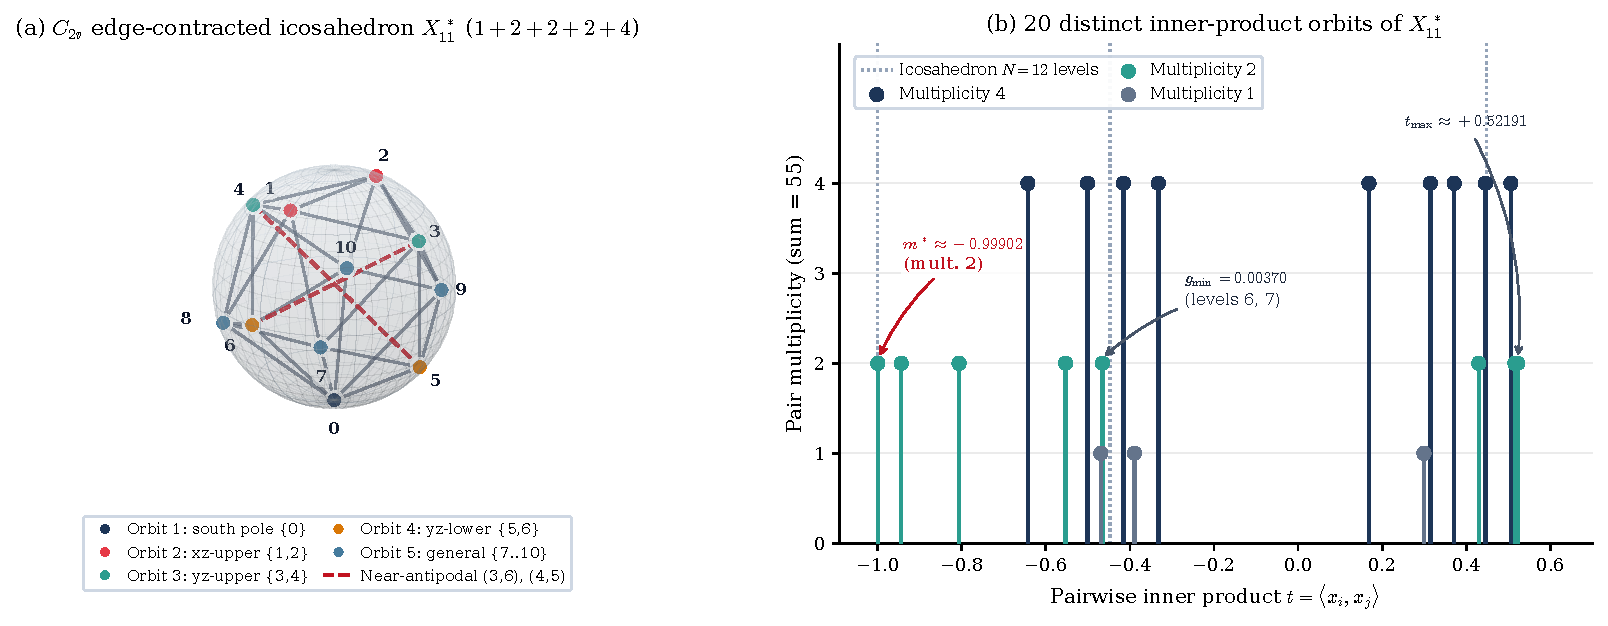
\includegraphics[width=\textwidth]{figures/fig_c2v.pdf}
  \caption{(a)~Three-dimensional rendering of the $C_{2v}$ edge-contracted icosahedron $\Xstar$ on $\Sph$, colored by its five symmetry orbits ($1+2+2+2+4$); dashed red chords mark the two disjoint nearly antipodal pairs $(3,6)$ and $(4,5)$ with inner product $m^* \approx -0.999023$. (b)~All $20$ distinct inner-product orbits of the $55$ pairs of $\Xstar$, compared with the three inner-product levels $\{-1, \pm 1/\sqrt{5}\}$ of the regular icosahedron ($N=12$).}
  \label{fig:c2v}
\end{figure}

\begin{table}[htbp]
  \centering
  \caption{The $20$ distinct pairwise inner-product orbits of $\Xstar$ ($\sum \mathrm{mult.} = 55$), computed at $80$-digit precision (\texttt{phase0\_candidate.json}). The tightest gap $g_{\min} = 0.0036973115$ lies between levels~$6$ and~$7$.}
  \label{tab:levels}
  \footnotesize
  \renewcommand{\arraystretch}{1.06}
  \begin{tabular}{@{}rrrl@{\qquad}rrrl@{}}
    \toprule
    Lvl & $\ip{x_i^*}{x_j^*}$ & Mult. & Orbit pairs & Lvl & $\ip{x_i^*}{x_j^*}$ & Mult. & Orbit pairs \\
    \midrule
    0 & $-0.9990227935$ & 2 & (3,6), (4,5) & 10 & $-0.3322522682$ & 4 & (5,8), (5,10), (6,7), (6,9) \\
    1 & $-0.9433100225$ & 2 & (7,10), (8,9) & 11 & $+0.1683597004$ & 4 & (0,7), (0,8), (0,9), (0,10) \\
    2 & $-0.8059548966$ & 2 & (0,1), (0,2) & 12 & $+0.2991265906$ & 1 & (1,2) \\
    3 & $-0.6423789841$ & 4 & (1,9), (1,10), (2,7), (2,8) & 13 & $+0.3144150202$ & 4 & (3,7), (3,9), (4,8), (4,10) \\
    4 & $-0.5526814629$ & 2 & (0,3), (0,4) & 14 & $+0.3709983342$ & 4 & (1,7), (1,8), (2,9), (2,10) \\
    5 & $-0.5005135913$ & 4 & (3,8), (3,10), (4,7), (4,9) & 15 & $+0.4294213841$ & 2 & (3,5), (4,6) \\
    6 & $-0.4689171004$ & 1 & (5,6) & 16 & $+0.4454363313$ & 4 & (1,3), (1,4), (2,3), (2,4) \\
    7 & $-0.4652197890$ & 2 & (7,9), (8,10) & 17 & $+0.5057661801$ & 4 & (5,7), (5,9), (6,8), (6,10) \\
    8 & $-0.4153143137$ & 4 & (1,5), (1,6), (2,5), (2,6) & 18 & $+0.5153071412$ & 2 & (0,5), (0,6) \\
    9 & $-0.3890864010$ & 1 & (3,4) & 19 & $+0.5219097664$ & 2 & (7,8), (9,10) \\
    \bottomrule
  \end{tabular}
\end{table}

\section{Elementary Milestones \texorpdfstring{\textnormal{\texttt{M0}}}{M0} and \texorpdfstring{\textnormal{\texttt{M1}}}{M1} in Lean~4}\label{sec:milestones}

Both frozen challenge statements in Listing~\ref{lst:challenge} admit short, direct proofs in \texttt{ThomsonN11/\allowbreak Solution.lean} requiring no external certificates:

\paragraph{Milestone \texttt{M0} ($E(x) \ge 55/2$).}
For any $x \in \mathrm{SphereConfig}(11)$ and $0 \le i < j < 11$, injectivity gives $0 < \norm{x_i - x_j} \le \norm{x_i} + \norm{x_j} = 2$, so $\norm{x_i - x_j}^{-1} \ge 1/2$. Summing over the $\binom{11}{2} = 55$ unordered pairs gives $E(x) \ge 55/2$ (\texttt{thomson\_eleven\_M0}, lines~61--88).

\paragraph{Milestone \texttt{M1} ($E(x) \ge 155/4$).}
Following Yudin's two-point linear programming method~\cite{Yudin1992}, consider the explicit rational quadratic polynomial (\texttt{fM1}, line~196)
\begin{equation}\label{eq:fM1}
  f_{M_1}(t) \;:=\; \frac{7}{10} + \frac{2}{5}t + \frac{7}{40}t^2.
\end{equation}
To certify $f_{M_1}(t) \le \varphi(t) = (2 - 2t)^{-1/2}$ on $[-1, 1)$, it suffices to show $1 - 2(1-t) f_{M_1}(t)^2 \ge 0$ on $[-1,1]$. In \texttt{fM1\_minorant\_nonneg} (lines~198--212), this is verified by an explicit rational $6$-square Luk\'acs identity:
\begin{align*}
  1 - 2(1-t) f_{M_1}(t)^2
  &= (1+t)\Biggl[
    \frac{1}{32}\!\left(-\frac{19}{40}+\frac{1291}{400}t+\frac{499}{400}t^2\right)^2 \\*
  &\qquad\qquad
    {}+ \frac{157279}{20480000}\!\left(\frac{4580}{157279}+\frac{305398}{157279}t-\frac{309978}{157279}t^2\right)^2 \\*
  &\qquad\qquad
    {}+ \frac{3053833}{503292800}(1-2t+t^2)^2
  \Biggr] \\
  &\quad + (1-t)\Biggl[
    \frac{11}{1600}\!\left(-\frac{17}{44}+\frac{29}{11}t+\frac{7}{4}t^2\right)^2 \\*
  &\qquad\qquad
    {}+ \frac{19}{11264}\!\left(\frac{146}{95}-\frac{102}{95}t-\frac{44}{95}t^2\right)^2 \\*
  &\qquad\qquad
    {}+ \frac{907}{486400}(1-2t+t^2)^2
  \Biggr] \;\ge\; 0,
\end{align*}
closed directly by \texttt{ring} and \texttt{positivity}.
Next, let $t_{ij} := \ip{x_i}{x_j}$. Since $\sum_{i,j} t_{ij} = \norm{\sum_i x_i}^2 \ge 0$ (\texttt{double\_sum\_dot\_nonneg}, line~214) and for $M_{ab} := \sum_i (x_i)_a (x_i)_b$ with $\operatorname{tr} M = 11$,
\[
  3\sum_{i,j} t_{ij}^2 - 11^2
  \;=\; (M_{00}-M_{11})^2 + (M_{11}-M_{22})^2 + (M_{22}-M_{00})^2 + 6(M_{01}^2 + M_{02}^2 + M_{12}^2) \;\ge\; 0
\]
(\texttt{double\_sum\_dot\_sq\_ge}, line~226), we have $\sum_{i,j} t_{ij}^2 \ge 121/3$.
Together with the diagonal sum $\sum_{i=0}^{10} f_{M_1}(1) = 11 \cdot \frac{51}{40} = \frac{561}{40}$, we obtain
\[
  E(x) \;\ge\; \frac{1}{2}\!\left(\sum_{i,j} f_{M_1}(t_{ij}) - \frac{561}{40}\right)
  \;\ge\; \frac{1}{2}\!\left(\frac{847}{10} + \frac{7}{40}\cdot\frac{121}{3} - \frac{561}{40}\right)
  \;=\; \frac{583}{15} \;=\; 38.866\ldots \;>\; \frac{155}{4},
\]
completing \texttt{thomson\_eleven\_M1} (lines~279--366).

\section{Three-Point SDP Universal Lower Bound (\texorpdfstring{\textnormal{\texttt{thomson\_eleven\_sdp\_M10}}}{thomson\_eleven\_sdp\_M10})}\label{sec:sdp-lb}

To push the Lean-certified lower bound from $38.75$ to $40.55547170437074$, we formalize an exact $S_3$-equivariant Bachoc--Vallentin / Cohn--Woo three-point semidefinite programming bound~\cite{BachocVallentin2008,CohnWoo2012} at order $(M,K) = (10,10)$ (polynomial degree $2M-2 = 18$).

\subsection{Three-point harmonic positivity and the \texorpdfstring{$11$}{11}-point \texorpdfstring{$S_3$}{S3} assembly identity}\label{subsec:assembly}
For $k \in \N$, define the Chebyshev--Gegenbauer three-point kernel $Q_k(u,v,t)$ recursively by $Q_0 = 1$, $Q_1(u,v,t) = t - uv$, and
\begin{equation}\label{eq:Qk}
  Q_{k+2}(u,v,t) \;=\; 2(t - uv)\,Q_{k+1}(u,v,t) - (1-u^2)(1-v^2)\,Q_k(u,v,t)
\end{equation}
(\texttt{StageB.Q3}, \texttt{ThreePoint.lean:141}).
Fixing any center $\xi \in \Sph$ and an orthonormal tangent frame $(e_1, e_2)$ orthogonal to $\xi$ (\texttt{exists\_ortho\_frame}, line~182), set $z_j := \ip{e_1}{x_j} + \sqrt{-1}\,\ip{e_2}{x_j} \in \C$.
Then $1 - \ip{\xi}{x_j}^2 = |z_j|^2$ and $\ip{x_j}{x_l} - \ip{\xi}{x_j}\ip{\xi}{x_l} = \operatorname{Re}(z_j \overline{z_l})$, so induction gives $Q_k(\ip{\xi}{x_j}, \ip{\xi}{x_l}, \ip{x_j}{x_l}) = \operatorname{Re}((z_j \overline{z_l})^k) = \operatorname{Re}(z_j^k)\operatorname{Re}(z_l^k) + \operatorname{Im}(z_j^k)\operatorname{Im}(z_l^k)$ (\texttt{Q3\_eq\_re}, line~147).
Choosing such an orthonormal frame $(e_1^{(i)}, e_2^{(i)})$ orthogonal to each $x_i$ and writing $z_{ij} := \ip{e_1^{(i)}}{x_j} + \sqrt{-1}\,\ip{e_2^{(i)}}{x_j}$, we obtain for any weight function $g : \R \to \R$:
\begin{align}\label{eq:bv-pos}
  \sum_{i=0}^{10}\sum_{j=0}^{10}\sum_{l=0}^{10}
  &g(\ip{x_i}{x_j})\,g(\ip{x_i}{x_l})\,Q_k(\ip{x_i}{x_j},\ip{x_i}{x_l},\ip{x_j}{x_l}) \nonumber \\
  &= \sum_{i=0}^{10}\!\left[\Bigl(\sum_{j=0}^{10} g(\ip{x_i}{x_j})\operatorname{Re}(z_{ij}^k)\Bigr)^2
    + \Bigl(\sum_{j=0}^{10} g(\ip{x_i}{x_j})\operatorname{Im}(z_{ij}^k)\Bigr)^2\right] \;\ge\; 0
\end{align}
(\texttt{sum\_Y3\_sq\_nonneg\_finset}, line~268).
Summing rank-$1$ weights $g(u) = \sum_{a=0}^{M-k-1} c_{k,r,a} u^a$ across integer Cholesky columns $r$ and harmonic orders $0 \le k < K$ yields a $(u \leftrightarrow v)$-symmetric polynomial $s(u,v,t)$ satisfying $\sum_{i,j,l} s(t_{ij}, t_{il}, t_{jl}) \ge 0$ for every unit-sphere configuration (\texttt{PolyKron.\allowbreak sum\_harmListEv\_nonneg}, \path{PolyKron.lean:1290}).

Let $\operatorname{sym}_3 s(u,v,t) := \frac{1}{6}\sum_{\pi \in S_3} s(\pi(u,v,t))$ and $g(u) := s(1,u,u) + s(u,1,u) + s(u,u,1)$.
For any symmetric $11\times 11$ matrix $(t_{ij})$ with unit diagonal $t_{ii} = 1$, any univariate polynomial $H : \R \to \R$, and any constant $e \in \R$, expanding the triple sum into diagonal ($11$ terms), $2$-point ($110$ ordered pairs), and distinct-triple ($990 = 6 \times 165$ ordered triples) strata gives the exact combinatorial identity (\texttt{StageB.cap\_assembly\_11}, \texttt{ThreePoint.lean:336}):
\begin{equation}\label{eq:cap-assembly-11}
  \sum_{0 \le i < j < 11} H(t_{ij}) - e
  \;=\; \frac{1}{3} \sum_{0 \le i < j < l < 11} \mathrm{slack}(t_{ij}, t_{il}, t_{jl})
  + \frac{1}{2} \sum_{i,j,l=0}^{10} s(t_{ij}, t_{il}, t_{jl}),
\end{equation}
where the $S_3$-symmetric triple slack polynomial is
\begin{equation}\label{eq:slack-def}
  \mathrm{slack}(u,v,t) \;:=\; \frac{H(u)+H(v)+H(t)}{3} - \frac{e}{55} - 9\,\operatorname{sym}_3 s(u,v,t) - \frac{g(u)+g(v)+g(t)}{3} - \frac{s(1,1,1)}{10}.
\end{equation}
Indeed, each of the $55$ unordered pairs lies in $9$ unordered triples (so $\frac{1}{3}\cdot\frac{9}{3} = 1$), and $\frac{1}{3}\cdot 165 = 55$, matching $55 \cdot (e/55) = e$ and $55 \cdot (s(1,1,1)/10) = \frac{11}{2} s(1,1,1)$.

\subsection{\texorpdfstring{$S_3$}{S3}-isotypic certificate and exact integer error accounting}\label{subsec:sdp-cert}
For any triple of unit vectors $(x_i, x_j, x_l)$, the pairwise inner products $(u,v,t) = (t_{ij}, t_{il}, t_{jl})$ lie in the compact semialgebraic domain
\[
  \mathcal{D}_3 \;:=\; \{(u,v,t) \in [-1,1]^3 : \det G(u,v,t) := 1 + 2uvt - u^2 - v^2 - t^2 \ge 0\}
\]
(\texttt{detG\_nonneg\_of\_unit}, \texttt{ThreePoint.lean:86}).
Exploiting the full $S_3$ permutation invariance of~\eqref{eq:slack-def}, we express the integer-scaled slack polynomial $1980\,S_2\,\mathrm{slack}(u,v,t)$ (where $S_2 := 2^{2B} = 2^{144}$ for Cholesky bit-precision $B = 72$, and $1980 = 6 \cdot \mathrm{lcm}(3, 55, 10)$ clears all rational denominators) as
\begin{equation}\label{eq:slack-sos}
  1980\,S_2\,\mathrm{slack}(u,v,t) \;=\; \Sigma_{\mathrm{cap}}(u,v,t) + r_{\mathrm{slack}}(u,v,t),
\end{equation}
where $\Sigma_{\mathrm{cap}}(u,v,t) \ge 0$ on $\mathcal{D}_3$ is a sum of $10$ integer-Cholesky sum-of-squares blocks decomposed by $S_3$ and $S_2$ isotypic components:
\begin{itemize}[leftmargin=2em,itemsep=1pt,topsep=3pt]
  \item $4$ one-dimensional $S_3$ blocks: trivial and sign representations on multipliers $1$ (sizes $53, 23$) and $\det G$ (sizes $31, 11$);
  \item $2$ two-dimensional $S_3$ standard representation blocks on multipliers $1$ (size $72$) and $\det G$ (size $39$);
  \item $4$ $S_2$-symmetric blocks (even/odd in $(v,t)$) on multipliers $1+u$ (sizes $95, 70$) and $1-u$ (sizes $95, 70$), summed over the $3$ cyclic permutations of $(u,v,t)$.
\end{itemize}
Because every block is stored directly as an integer Cholesky factor $C$ (evaluating $\sum_r (C_r^\top b)^2$ with zero diagonal-dominance remainder), nonnegativity $\Sigma_{\mathrm{cap}} \ge 0$ on $\mathcal{D}_3$ follows immediately from \texttt{sq\_nonneg} (\texttt{SdpCert.sosCap\_ev\_nonneg}, \texttt{SdpCert.lean:361}).
The integer residual polynomial $r_{\mathrm{slack}}$ has $1{,}330 = \binom{21}{3}$ nonzero monomials (split into $14$ chunks in \path{SdpCertSosData.lean}) and satisfies $|r_{\mathrm{slack}}(u,v,t)| \le \norm{r_{\mathrm{slack}}}_1$ on $[-1,1]^3$, with
\[
  R_{\mathrm{slack}} \;:=\; \frac{\norm{r_{\mathrm{slack}}}_1}{1980\,S_2} \;\approx\; 4.334 \times 10^{-18}.
\]

For the univariate Coulomb minorant $H(t) = H_{\mathrm{int}}(t)/S_2 \le (1 + R_y)\varphi(t)$ on $t \in [-1,1)$, we substitute $y := \sqrt{(1-t)/2} \in (0,1]$, so $t = 1 - 2y^2$ and $\varphi(t) = (2y)^{-1}$.
The module \texttt{SdpCertHarmData.lean} stores four integer Cholesky 1D SOS tables $\sigma_0,\sigma_1,\sigma_2,\sigma_3$ and a $38$-term integer residual $r_y(y)$ verifying identically (\texttt{minor\_ok}, line~197)
\begin{equation}\label{eq:minorant-1d}
  2y\,H_{\mathrm{int}}(1 - 2y^2) - S_2 + \sigma_0(y) + y\,\sigma_1(y) + (1-y^2)\sigma_2(y) + y(1-y^2)\sigma_3(y) - r_y(y) \;=\; 0,
\end{equation}
yielding $H(t) \le (1 + R_y)\varphi(t)$ with $R_y := \norm{r_y}_1 / S_2 \approx 3.587 \times 10^{-17}$ (\texttt{SdpCert.minorCap\_bound}, \texttt{SdpCert.lean:397}).

Combining~\eqref{eq:bv-pos}, \eqref{eq:cap-assembly-11}, \eqref{eq:slack-sos}, and~\eqref{eq:minorant-1d} with $e_{\mathrm{int}}/S_2 = 40.5554717043707436\ldots$ gives, for every $x \in \mathrm{SphereConfig}(11)$,
\[
  (1 + R_y)\,E(x) \;\ge\; \sum_{0 \le i < j < 11} H(t_{ij})
  \;\ge\; \frac{e_{\mathrm{int}}}{S_2} - 55\,R_{\mathrm{slack}}
  \;=\; \frac{36\,e_{\mathrm{int}} - \norm{r_{\mathrm{slack}}}_1}{36\,S_2},
\]
since $55 / 1980 = 1/36$.
The exact integer cross-multiplied inequality (\texttt{SdpCertSosData.bound\_ok}, line~1425)
\[
  2027773585218537 \cdot 36 \cdot \bigl(S_2 + \norm{r_y}_1\bigr)
  \;\le\; 50000000000000 \cdot \bigl(36\,e_{\mathrm{int}} - \norm{r_{\mathrm{slack}}}_1\bigr)
\]
is checked directly by \texttt{decide +kernel} (the unrounded ratio equals $40.5554717043707419\ldots$, leaving a clean safety margin of $1.92 \times 10^{-15}$ above $\Elb$), proving \texttt{SdpCert.global\_sdp\_lower\_bound} (\texttt{SdpCert.lean:435}) and hence~\eqref{eq:sdp-lb} (\texttt{Solution.lean:373}).

\section{Pure-Integer Projective Stereographic Upper Bound}\label{sec:upper}

Formalizing tight upper bounds for $N = 11$ requires care because $\Xstar$ has irrational coordinates involving no closed-form algebraic expression.
Rather than wrapping floating-point coordinates in interval square roots, we exploit the rational stereographic parameterization~\eqref{eq:stereo}--\eqref{eq:c2v-orbits} in \path{numerics/bounds/export_lean_upper.py} and \path{StageB/UpperBound.lean}:

\begin{enumerate}[leftmargin=2.2em]
  \item \emph{Zero-square-root rational points on $\Sph$.} Rounding the $80$-digit stationary parameters $(t_1^*, t_2^*, t_3^*, u_4^*, v_4^*)$ to denominator $10^9$ gives five exact rationals:
  \[
    t_1 = \frac{40973957}{125000000},\quad
    t_2 = \frac{536744081}{1000000000},\quad
    t_3 = \frac{221017691}{125000000},\quad
    u_4 = \frac{514601287}{500000000},\quad
    v_4 = \frac{73487661}{125000000}.
  \]
  Clearing denominators in~\eqref{eq:stereo} yields $11$ integer projective quadruples $(X_i, Y_i, Z_i, D_i) \in \Z^4$ (\texttt{c2vPtsZ}, lines~22--34) satisfying $D_i > 0$ and the exact Pythagorean identity $X_i^2 + Y_i^2 + Z_i^2 = D_i^2$ (\texttt{unit\_ok}, line~62), so $x_i^{\mathrm{wit}} := (X_i/D_i, Y_i/D_i, Z_i/D_i)$ lies \emph{identically} on $\Sph$ (\texttt{c2vWitness\_unit}, line~88).
  Because $\Xstar$ is a stationary point ($\nabla_{\Sph} E(\Xstar) = 0$), an $O(10^{-9})$ parameter rounding perturbs the Coulomb energy only at second order: $E(x^{\mathrm{wit}}) - E^*(11) \approx 1.78 \times 10^{-18}$ ($E(x^{\mathrm{wit}}) = 40.59645050819060538841\ldots$).
  \item \emph{Pure-$\Z$ inverse-distance upper certification.} Set $S_{\mathrm{inv}} := 5 \times 10^{16}$ and, for each $0 \le i < j < 11$, define the integer squared chord numerator
  \[
    \mathrm{distNumSq}_Z(i,j) \;:=\; (X_i D_j - X_j D_i)^2 + (Y_i D_j - Y_j D_i)^2 + (Z_i D_j - Z_j D_i)^2 \;=\; D_i^2 D_j^2 \norm{x_i^{\mathrm{wit}} - x_j^{\mathrm{wit}}}^2.
  \]
  We precompute the smallest positive integers $u_{ij}$ (\texttt{uUpperZ}, lines~36--48) such that
  \begin{equation}\label{eq:upper-int}
    u_{ij} > 0
    \qquad\text{and}\qquad
    S_{\mathrm{inv}}^2 D_i^2 D_j^2 \;\le\; u_{ij}^2\,\mathrm{distNumSq}_Z(i,j).
  \end{equation}
  Checking~\eqref{eq:upper-int} across all $55$ pairs via a single pure-$\Z$ \texttt{decide +kernel} call (\texttt{pair\_u\_ok}, line~66) simultaneously proves both injectivity of $x^{\mathrm{wit}}$ (since $S_{\mathrm{inv}} > 0$ rules out $\norm{x_i^{\mathrm{wit}} - x_j^{\mathrm{wit}}} = 0$, \texttt{c2vWitness\_injective}, line~150) and the pairwise upper bound $\norm{x_i^{\mathrm{wit}} - x_j^{\mathrm{wit}}}^{-1} \le u_{ij} / S_{\mathrm{inv}}$.
  Finally, \texttt{energy\_sum\_ok} (line~74) checks
  \[
    \sum_{0 \le i < j < 11} u_{ij} \;=\; 2029822525409530294 \;\le\; 2029822525409531000 \;=\; S_{\mathrm{inv}} \cdot \Eub,
  \]
  yielding $E(x^{\mathrm{wit}}) \le 40.59645050819060588 \le \Eub = 40.59645050819062$ (\texttt{c2vWitness\_energy\_le}, line~162) in under $15\,\mathrm{s}$ of kernel time with zero rational GCD overhead.
\end{enumerate}

\section{Stage~A Exact Rational Ladder and the Three-Point SDP Obstruction}\label{sec:obstruction}

Why does Theorem~\ref{thm:main} stop at a gap of $0.0410$, whereas the exact same $S_3$-equivariant $(10,10)$ three-point SDP formulation closes $N = 9$ to within $1.2 \times 10^{-17}$~\cite{Li2026N9}?
In this section we present the complete Stage~A computational evidence (\texttt{numerics/bounds/verify\_all.py}, \texttt{phase0\_sdp\_sweep.py}, \texttt{phase0\_gap\_diagnosis.py}) demonstrating that $N = 11$ exhibits an \emph{intrinsic} positive three-point relaxation gap $\Delta \approx 0.0395$ caused by a fractional-icosahedral dual pseudo-measure.

\subsection{Fifteen exact rational Stage~A certificates up to \texorpdfstring{$(M,K) = (12,12)$}{(M,K) = (12,12)}}\label{subsec:stagea-ladder}
Using our pure-\texttt{Fraction} $S_3$ cap engine (\texttt{sym\_cap\_sdpa.py}, uncapped harmonic order $K = M$) and $(2,9)$-typed pole-ring strip engine (\texttt{sym\_strip\_sdpa.py}), solved in $200/224$-bit \texttt{SDPA-GMP} and verified out of process via exact integer Bareiss Sylvester sequential principal minors (\texttt{exact\_linalg.py}, zero floating-point trust, polynomial identity error identically~$0$), we generated and verified $15$ exact rational certificates totaling $410$ positive-definite blocks; Table~\ref{tab:certs} summarizes the entire suite.

\begin{table}[htbp]
  \centering
  \caption{All $15$ independently verified exact rational Stage~A certificates in \texttt{certificates/} ($410$ positive-definite blocks total; exact Bareiss PD check passed and combinatorial identity error $= 0$ on every file). Values are displayed to $12$ decimal places from \texttt{verify\_all.json}; $\Delta := E^*(11) - e_{\mathrm{cert}}$.}
  \label{tab:certs}
  \footnotesize
  \renewcommand{\arraystretch}{1.08}
  \begin{tabular}{@{}lrrrrrr@{}}
    \toprule
    Model \& inner-product domain & $(M,K)$ & Deg. & Blocks & Solve (s) & $e_{\mathrm{cert}}$ & Gap $\Delta$ \\
    \midrule
    Global $S_3$, $t \in [-1, 1]$ & $(6,6)$ & 10 & 20 & $5.4$ & $40.533315701817$ & $0.063135$ \\
    Global $S_3$, $t \in [-1, 1]$ & $(7,7)$ & 12 & 21 & $14.5$ & $40.545314785703$ & $0.051136$ \\
    Global $S_3$, $t \in [-1, 1]$ & $(8,8)$ & 14 & 22 & $89.0$ & $40.551494289332$ & $0.044956$ \\
    Global $S_3$, $t \in [-1, 1]$ & $(9,9)$ & 16 & 23 & $214.1$ & $40.554160636831$ & $0.042290$ \\
    \textbf{Global $S_3$, $t \in [-1, 1]$ (Lean~4)} & $\mathbf{(10,10)}$ & \textbf{18} & \textbf{24} & $\mathbf{1145.0}$ & $\mathbf{40.555471704371}$ & $\mathbf{0.040979}$ \\
    \textbf{Global $S_3$, $t \in [-1, 1]$ (best global)} & $\mathbf{(12,12)}$ & \textbf{22} & \textbf{26} & $\mathbf{9541.6}$ & $\mathbf{40.556960329409}$ & $\mathbf{0.039490}$ \\
    \midrule
    Lower cap $S_3$, $t \in [-1023/1024, 1]$ & $(6,6)$ & 10 & 20 & $5.5$ & $40.533320366836$ & $0.063130$ \\
    Lower cap $S_3$, $t \in [-1023/1024, 1]$ & $(8,8)$ & 14 & 22 & $106.5$ & $40.551516085750$ & $0.044934$ \\
    Lower cap $S_3$, $t \in [-1023/1024, 1]$ & $(10,10)$ & 18 & 24 & $1148.8$ & $40.555539579695$ & $0.040911$ \\
    Lower cap $S_3$, $t \in [-1023/1024, 1]$ & $(12,12)$ & 22 & 26 & $9608.9$ & $40.556970864736$ & $0.039480$ \\
    Upper cap $S_3$, $t \in [-1, 53/100]$ & $(8,8)$ & 14 & 24 & $122.9$ & $40.551787212256$ & $0.044663$ \\
    Deep cap $S_3$, $t \in [-49/50, 1]$ & $(8,8)$ & 14 & 22 & $51.5$ & $40.554952399256$ & $0.041498$ \\
    Strong cap $S_3$, $t \in [-9/10, 1]$ & $(8,8)$ & 14 & 22 & $49.1$ & $40.584934945776$ & $0.011516$ \\
    \midrule
    $(2,9)$ strip, $t_{01} \in [-1, -1023/1024]$ & $(6,6)$ & 10 & 56 & $66.3$ & $40.536870920686$ & $0.059580$ \\
    $(2,9)$ strip, $t_{01} \in [-9991/10000, -999/1000]$ & $(7,7)$ & 12 & 58 & $312.6$ & $40.548003495494$ & $0.048447$ \\
    \bottomrule
  \end{tabular}
\end{table}

Three empirical facts jump out from Table~\ref{tab:certs} and Figure~\ref{fig:obstruction}(a):
\begin{enumerate}[leftmargin=2.2em]
  \item \emph{Rapid saturation well below $E^*(11)$.} Along the global $a_0 = -1$ ladder, consecutive increments decay sharply: $+0.01200$ from $(6,6)$ to $(7,7)$, $+0.00618$ to $(8,8)$, $+0.00267$ to $(9,9)$, $+0.00131$ to $(10,10)$, and only $+0.00149$ across the two-step jump from $(10,10)$ to $(12,12)$ (at an $8.3\times$ solve-time increase to $9{,}542\,\mathrm{s}$).
  \item \emph{Icosahedral harmonic parity selection rule at $(12,12)$.} Inspecting the certified harmonic block traces $\operatorname{tr} F_k$ of the $(12,12)$ certificate (\texttt{phase0\_gap\_diagnosis.json}) shows $F_0, \dots, F_8$ active ($\operatorname{tr} F_8 = 2.06 \times 10^{-2}$), the \emph{odd} orders strictly inactive ($\operatorname{tr} F_9 = 3.44 \times 10^{-20}$, $\operatorname{tr} F_{11} = 5.72 \times 10^{-23}$), and the \emph{even} order $F_{10}$ active ($\operatorname{tr} F_{10} = 1.05 \times 10^{-4}$). This matches the exact spherical-harmonic invariant degrees $\ell \in \{0, 6, 10, 12, \dots\}$ of the icosahedral group $I_h$ (which admits no invariants at $\ell = 9$ or $\ell = 11$).
  \item \emph{Ineffectiveness of cap cuts and $(2,9)$ pole-ring strips.} Cutting below $m^*$ at $a_0 = -1023/1024 \approx -0.9990234$ raises the $(12,12)$ bound by only $+1.05 \times 10^{-5}$ to $40.556971$. Cutting above $t_{\max}$ at $b_0 = 53/100$ adds $+2.93 \times 10^{-4}$ at $(8,8)$. Even an aggressive cap $a_0 = -9/10$---which excludes both $m^*$ and level~$1$ ($-0.9433$) of $\Xstar$ itself---still certifies only $40.584935 < E^*(11)$. Likewise, our $(2,9)$-typed pole-ring strip SDP (whose Lean combinatorial assembly identity is already formalized in \texttt{StageB.slab\_assembly\_11}, \texttt{ThreePoint.lean:770}) achieves only $40.536871$ on $[-1, -1023/1024]$ at $(6,6)$ and $40.548003$ on the narrow strip $[-9991/10000, -999/1000] \ni m^*$ at $(7,7)$.
\end{enumerate}

\begin{figure}[htbp]
  \centering
  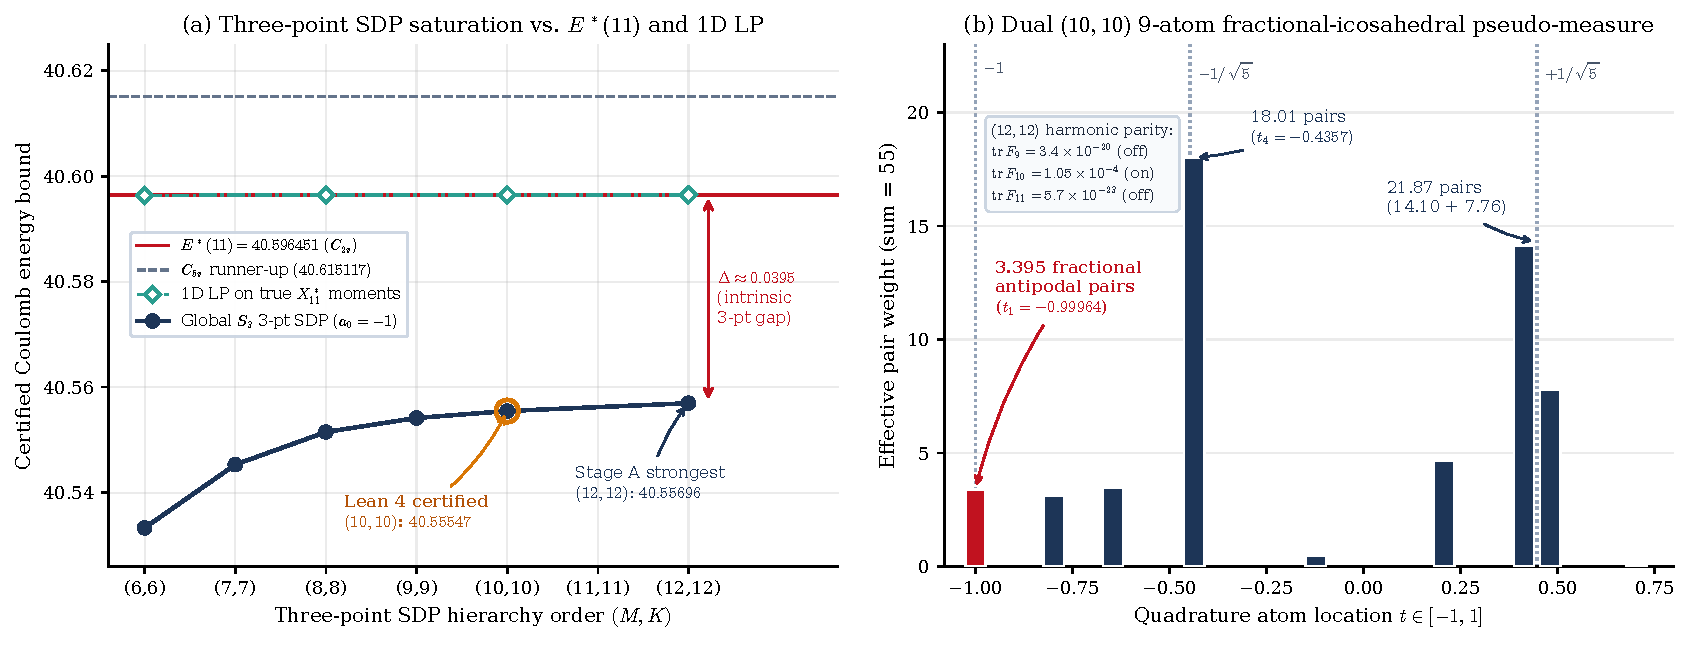
\includegraphics[width=\textwidth]{figures/fig_sdp_obstruction.pdf}
  \caption{(a)~Saturation of the exact rational global $S_3$ three-point SDP ladder across $(M,K) = (6,6)\dots(12,12)$ versus the $C_{2v}$ optimum $E^*(11)$, the $C_{5v}$ runner-up, and the discrete-grid $1\text{D}$ minorant LP on true $\Xstar$ moments. (b)~The optimal $(10,10)$ dual $9$-atom Gauss--Christoffel pseudo-measure (effective pair weights summing to $55$), showing $3.395$ fractional antipodal pairs at $t_1 = -0.99964$ and $18.01$ / $21.87$ icosahedral-angle pairs near $\mp 1/\sqrt{5}$, together with the $(12,12)$ icosahedral harmonic parity rule.}
  \label{fig:obstruction}
\end{figure}

\subsection{First-principles diagnosis: fractional-icosahedral pseudo-moments}\label{subsec:diagnosis}
To pinpoint the root cause of the $\Delta \approx 0.0395$ plateau, \texttt{phase0\_gap\_diagnosis.py} performs three independent tests:

\paragraph{Test 1: Ruling out polynomial degree via a 1D true-moment LP.}
Fixing the exact $20$-level pair distribution of $\Xstar$ from Table~\ref{tab:levels}, we maximize $\sum_{i<j} H(t^*_{ij})$ over degree-$(2M-2)$ polynomials $H$ subject to $2y\,H(1-2y^2) \le 1$ on a $20{,}001$-point grid in $y \in [10^{-4}, 1]$.
This discrete-grid LP achieves $40.586405$ at $M = 4$ ($\deg H = 6$), $40.596353$ at $M = 6$ ($\deg H = 10$), and $40.59645006$ at $M = 8$ ($\deg H = 14$, gap $4.52 \times 10^{-7}$), saturating to within $O(10^{-8})$ grid discretization error at $M = 10, 12$.
Hence polynomial approximation degree is \emph{not} the bottleneck: even degree~$14$ separates $\Xstar$ five orders of magnitude more tightly than the degree-$22$ three-point SDP.

\paragraph{Test 2: Spectral reconstruction of the $(10,10)$ dual pseudo-measure.}
Solving the $(10,10)$ dual SDP yields marginal pair pseudo-moments $(\mu_0, \dots, \mu_{18})$ whose $10 \times 10$ Hankel matrix is strictly positive definite (smallest eigenvalue $2.20 \times 10^{-8}$).
Table~\ref{tab:atoms} and Figure~\ref{fig:obstruction}(b) present its $9$-atom Gauss--Christoffel quadrature reconstruction (total effective pair count $55$).
Comparing against the $12$-vertex regular icosahedron---whose $66$ pairs consist of $6$ antipodal pairs at $-1$, $30$ pairs at $-1/\sqrt{5} \approx -0.4472$, and $30$ pairs at $+1/\sqrt{5} \approx +0.4472$---reveals the geometric identity of the spurious dual optimum: it places $3.3946$ \emph{fractional antipodal pairs} at $t_1 = -0.999637$ (with exact primal contact $\varphi(-1) - H^*(-1) = 5.0 \times 10^{-16}$), $18.0106$ pairs at $t_4 = -0.435716 \approx -1/\sqrt{5}$, and $14.1025 + 7.7630 = 21.8655$ pairs straddling $+1/\sqrt{5}$.
Moreover, its global Gram traces ($\operatorname{Tr} G^2 = 40.3718$, $\operatorname{Tr} G^3 = 148.2835$) match those of $\Xstar$ ($\operatorname{Tr} G^2 = 40.3689$, $\operatorname{Tr} G^3 = 148.2822$) to within $0.008\%$.

\begin{table}[htbp]
  \centering
  \caption{Optimal $(10,10)$ dual $9$-atom Gauss--Christoffel quadrature pseudo-measure (effective pair weights summing to $55$, \texttt{phase0\_gap\_diagnosis.json}).}
  \label{tab:atoms}
  \footnotesize
  \renewcommand{\arraystretch}{1.06}
  \begin{tabular}{@{}rrrr@{\qquad}rrrr@{}}
    \toprule
    Atom & Location $t_r$ & Eff.\ pairs & $\varphi(t_r)$ & Atom & Location $t_r$ & Eff.\ pairs & $\varphi(t_r)$ \\
    \midrule
    1 & $-0.999637$ & $\mathbf{3.3946}$ & $0.500045$ & 6 & $+0.208297$ & $4.6301$ & $0.794701$ \\
    2 & $-0.798561$ & $3.1281$ & $0.527257$ & 7 & $+0.413865$ & $\mathbf{14.1025}$ & $0.923605$ \\
    3 & $-0.645679$ & $3.4801$ & $0.551204$ & 8 & $+0.481741$ & $\mathbf{7.7630}$ & $0.982226$ \\
    4 & $-0.435716$ & $\mathbf{18.0106}$ & $0.590134$ & 9 & $+0.703210$ & $0.0071$ & $1.297958$ \\
    5 & $-0.123068$ & $0.4840$ & $0.667240$ & & \textbf{Sum} & $\mathbf{55.0000}$ & \\
    \bottomrule
  \end{tabular}
\end{table}

\paragraph{Test 3: True $\R^3$ $k$-antipodal energy ladder and dual lock-in.}
Why cannot a single-pair $(2,9)$ strip exclude the near-antipodal region as it did for $N = 9$~\cite{Li2026N9}?
Optimizing $11$ points on $\Sph$ subject to $k \in \{0,1,2,3,4,5\}$ forced exact antipodal pairs $x_{2r-1} = -x_{2r}$ ($40$ random starts per $k$, \texttt{phase0\_gap\_diagnosis.py}) produces the energy barrier plotted in Figure~\ref{fig:4pt}(a):
\begin{center}
\footnotesize
\begin{tabular}{@{}lrrrrrr@{}}
  \toprule
  Exact antipodal pairs $k$ & $0$ & $1$ & $2$ & $3$ & $4$ & $5$ \\
  \midrule
  True $\Sph$ min $E_{\min}(k)$ & $40.596451$ & $40.596907$ & $40.597677$ & $40.625784$ & $40.780435$ & $40.900671$ \\
  Penalty $E_{\min}(k) - E^*(11)$ & $0$ & $+0.000457$ & $+0.001227$ & $+0.029334$ & $+0.183984$ & $+0.304221$ \\
  \bottomrule
\end{tabular}
\end{center}
This uncovers a \emph{dual lock-in mechanism}:
(a)~because genuine spherical $11$-point configurations with $k = 1$ or $k = 2$ antipodal pairs sit only $+4.57 \times 10^{-4}$ and $+1.23 \times 10^{-3}$ above $E^*(11)$, any single-pair $(2,9)$ slab near $t = -1$ has a true geometric ceiling at $40.59691$ and cannot achieve large exclusion margins;
(b)~simultaneously, three-point SDP enforces only $3\times 3$ Gram positivity ($\det G_3 \ge 0$) and three-point harmonic PSD constraints, remaining blind to the four-point Euclidean rank-$3$ realizability identity $\det G_4 = 0$ (formalized in \texttt{StageB.det4\_eq\_zero\_of\_unit}, \texttt{ThreePoint.lean:105}).
As Figure~\ref{fig:4pt}(a) illustrates, the dual pseudo-measure tunnels directly beneath the steep $k \ge 3$ three-dimensional frustration wall at $k_{\mathrm{eff}} = 3.395$, smearing the single missing vertex of the icosahedron across $\approx 3.4$ fractional antipodal pairs without paying the $+0.03$ to $+0.18$ geometric frustration cost required in $\R^3$.

\section{Coupled \texorpdfstring{$S_{11} \times O(3)$}{S11 x O(3)} Four-Point SDP Probe and Closure Roadmap}\label{sec:fourpoint}

A natural question is whether adjoining four-point constraints---most notably the Euclidean realizability ideal $\det G_4 = 0$ and four-point $O(3)$-invariant positive-semidefinite blocks---breaks the $\approx 40.557$ ceiling at tractable polynomial degrees.
To test this quantitatively, we implemented an exact rational $S_{11} \times O(3)$-reduced coupled three-point + four-point SDP hierarchy probe in \path{numerics/bounds/phase0_4pt_probe.py} (ledger \path{results/phase0_4pt_probe.json}).

\subsection{Classification of \texorpdfstring{$S_{11} \times O(3)$}{S11 x O(3)}-invariant four-point blocks}\label{subsec:4pt-blocks}
For any $4$-tuple of distinct points $(x_0, x_1, x_2, x_3)$ on $\Sph$, let $e = (t_{01}, t_{02}, t_{03}, t_{12}, t_{13}, t_{23})$ denote its six pairwise inner products.
Up to edge-monomial degree $D_4$, our probe couples the full $S_3$ three-point SDP of degree $D_3 = 2M - 2$ with all three representation-theoretic families of $S_{11} \times O(3)$-invariant four-point constraints:
\begin{enumerate}[leftmargin=2.2em]
  \item \emph{Case 4 (4 free vertices):}
  (i)~exact $\R^3$ realizability ideal multipliers $q(e)\det G_4(e) = 0$ ($\deg q \le D_4 - 4$);
  (ii)~$\Z_2 \times \Z_2 = \langle(01),(23)\rangle$-block-diagonalized four-point Putinar SOS on multipliers $1$, $1+t_{01}$, $1-t_{01}$; and
  (iii)~$\Z_2 = \langle(01)\rangle$-block-diagonalized face-Gram SOS on $\det G_3(t_{01}, t_{02}, t_{12}) \ge 0$.
  \item \emph{Case 2 (2 free vertices + 1 summed neighbor):}
  (i)~Binet--Cauchy odd-parity cross-product block \texttt{Harm4\_odd}, arising from $\sum_{i\ne j} s_{ij} s_{ij}^\top \succeq 0$ with $s_{ij} = \sum_k w(t_{ij}, t_{ik}, t_{jk})\,((x_i \times x_j)\cdot x_k)$; and
  (ii)~even-parity pair-flag block \texttt{Flag2\_even} ($\sum_{i \ne j} f_{ij} f_{ij}^\top \succeq 0$).
  \item \emph{Case 0 (0 free vertices + 2 summed vertices):}
  global pair-tensor blocks \texttt{GlobNat\_d}$d$ ($0 \le d \le D_4$) and \texttt{GlobAx\_d}$d$ ($2 \le d \le D_4 - 1$) in $(\R^3)^{\otimes d}$, explicitly coupling disjoint pairs $(i,j),(k,m)$, $3$-edge paths $j\text{--}i\text{--}k\text{--}m$, and ambient dimension contractions $\|I_3\|^2 = 3$.
\end{enumerate}
Before every solve, all LP columns and PSD block entries are verified with \emph{zero} exact \texttt{Fraction} error against explicit geometric evaluation on a random rational $11$-point sphere configuration.

\subsection{Empirical results and resolution threshold}\label{subsec:4pt-results}
Table~\ref{tab:4pt} and Figure~\ref{fig:4pt}(b) summarize all $8$ \texttt{SDPA-GMP} runs (\texttt{pdOPT} on every run).

\begin{figure}[htbp]
  \centering
  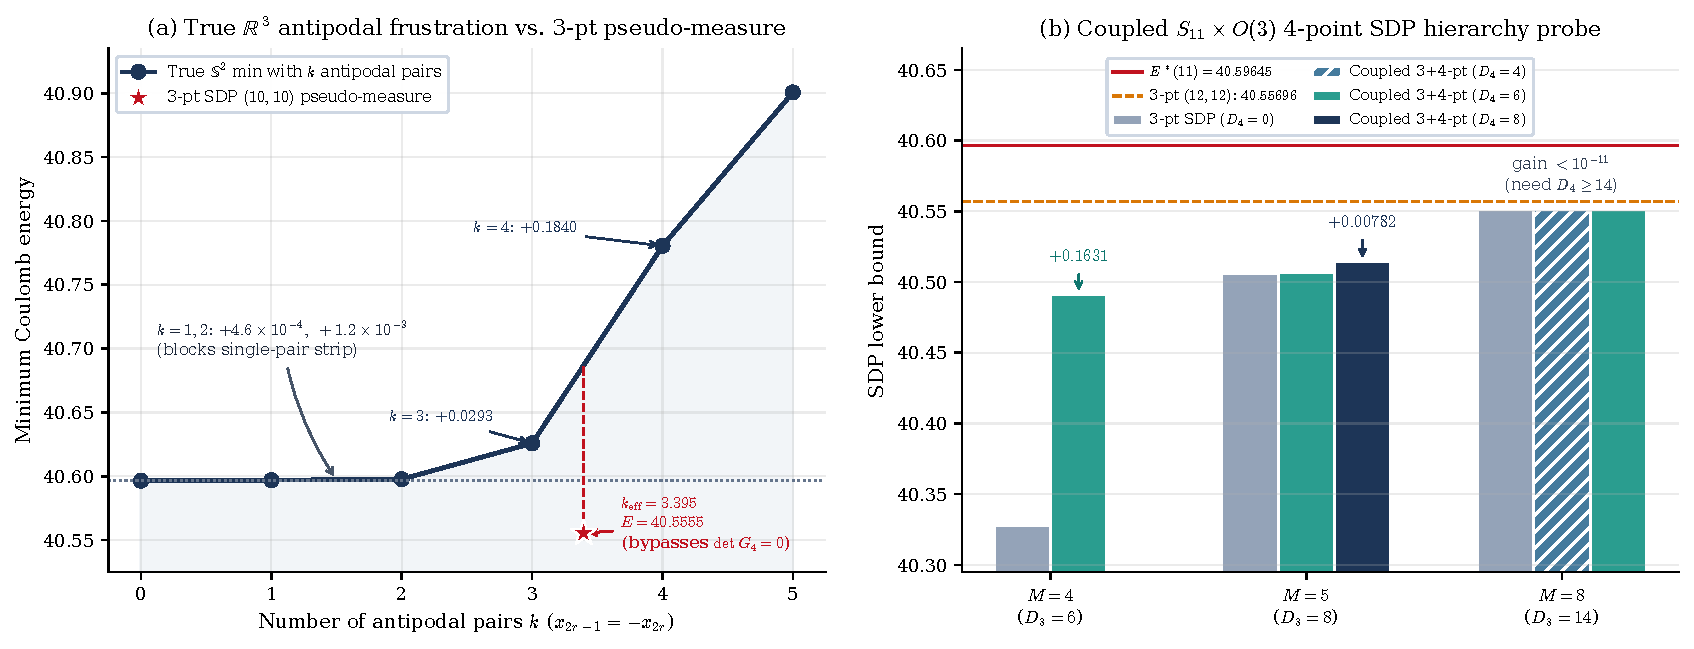
\includegraphics[width=\textwidth]{figures/fig_4pt_probe.pdf}
  \caption{(a)~True $\Sph$ minimum energy with $k \in \{0,\dots,5\}$ forced antipodal pairs versus the $(10,10)$ three-point SDP dual pseudo-measure ($k_{\mathrm{eff}} = 3.395$, $E = 40.5555$), showing how three-point SDP tunnels beneath the $k \ge 3$ three-dimensional frustration wall. (b)~Coupled $S_{11} \times O(3)$ four-point SDP hierarchy probe across $(M, D_3) \in \{(4,6), (5,8), (8,14)\}$.}
  \label{fig:4pt}
\end{figure}

\begin{table}[htbp]
  \centering
  \caption{Coupled $S_{11} \times O(3)$ three-point + four-point SDP probe results (\texttt{phase0\_4pt\_probe.json}, all runs \texttt{pdOPT}).}
  \label{tab:4pt}
  \footnotesize
  \renewcommand{\arraystretch}{1.08}
  \begin{tabular}{@{}rrrrrrrrr@{}}
    \toprule
    $(M,K)$ & $D_3$ & $D_4$ & Rows $m$ & Blocks & Entries & Solve (s) & Lower bound $e_{\mathrm{raw}}$ & Gain vs.\ 3-pt \\
    \midrule
    $(4,4)$ & 6 & 0 & 37 & 18 & 636 & $0.17$ & $40.32802558$ & $0$ \\
    $(4,4)$ & 6 & 6 & 86 & 45 & 10{,}021 & $9.48$ & $40.49109850$ & $\mathbf{+0.16307292}$ \\
    \midrule
    $(5,5)$ & 8 & 0 & 59 & 19 & 1{,}700 & $0.67$ & $40.50635763$ & $0$ \\
    $(5,5)$ & 8 & 6 & 108 & 46 & 11{,}085 & $9.34$ & $40.50651291$ & $+0.00015528$ \\
    $(5,5)$ & 8 & 8 & 213 & 50 & 115{,}414 & $352.93$ & $40.51417969$ & $\mathbf{+0.00782206}$ \\
    \midrule
    $(8,8)$ & 14 & 0 & 177 & 23 & 22{,}690 & $50.57$ & $40.55149429$ & $0$ \\
    $(8,8)$ & 14 & 4 & 188 & 45 & 23{,}522 & $56.85$ & $40.55149429$ & $< 10^{-12}$ \\
    $(8,8)$ & 14 & 6 & 226 & 50 & 32{,}075 & $70.80$ & $40.55149429$ & $< 10^{-11}$ \\
    \bottomrule
  \end{tabular}
\end{table}

Two clear conclusions emerge:
\begin{enumerate}[leftmargin=2.2em]
  \item \emph{Strict matched-degree strengthening.} At equal polynomial degrees $D_3 = D_4$, four-point constraints substantially beat three-point SDP: $+0.163073$ at degree~$6$ ($M=4$) and $+0.007822$ at degree~$8$ ($M=5$).
  \item \emph{Resolution bottleneck at $D_4 \le 8$.} Coupling low-degree four-point constraints ($D_4 \in \{4, 6\}$) onto high-degree three-point SDP ($M = 8, D_3 = 14$, bound $40.551494$) produces zero lift ($< 10^{-11}$). Thus the $9$-atom fractional-icosahedral pseudo-measure of Table~\ref{tab:atoms} admits a feasible degree-$6$ four-point moment extension satisfying $\det G_4 = 0$ and all Case~0/2/4 PSD constraints.
\end{enumerate}

\subsection{Roadmap toward a complete proof for \texorpdfstring{$N = 11$}{N = 11}}\label{subsec:roadmap}
Our diagnosis points to two concrete paths capable of closing the remaining $0.0395$ gap:
\begin{itemize}[leftmargin=2em]
  \item \emph{Full $S_4$-isotypic high-degree four-point SDP ($D_4 \ge 14\text{--}18$).} Replacing our $\Z_2 \times \Z_2$ symmetry reduction with full $S_4$ irreducible-representation block-diagonalization compresses the $6$-variable four-point SOS and tensor blocks by roughly $6\times$, bringing $D_4 \ge 14$---the polynomial resolution needed to separate the $9$ dual pseudo-atoms---within reach of high-precision SDP solvers.
  \item \emph{Multi-pair matching branch-and-bound + SDP pruning.} Instead of splitting on a single minimum inner product, branch on the matching number $k \in \{0, 1, 2, \ge 3\}$ of the near-antipodal graph $G_{\le -0.95}$: configurations with $k \ge 3$ face a $+0.0293$ to $+0.3042$ energy penalty amenable to $(2k, 11-2k)$-typed multi-pole SDP exclusion; the low-dimensional $k = 1, 2$ strata have reduced geometric degrees of freedom suited to interval branch-and-bound; and the $k = 0$ basin closes locally around the $5$-parameter $C_{2v}$ stationary point $\Xstar$ via a Krawczyk existence-uniqueness operator and a $33 \times 33$ integer-Cholesky Riemannian Hessian bound (since $\lambda_{\min}(H_0) \approx 0.0907 > 0$).
\end{itemize}

\section{Lean~4 Kernel Architecture, Verification Record, and Discussion}\label{sec:lean}

Nothing about \texttt{SDPA-GMP} or the Python certificate exporters is trusted in Theorem~\ref{thm:main}; every algebraic identity, positivity statement, and rational inequality is checked from scratch inside the Lean~4 kernel.

\subsection{Zero-Mathlib \texorpdfstring{\texttt{Init}}{Init} data layer and \texorpdfstring{$19$}{19}-slice \texorpdfstring{$2\text{D}$}{2D}-Kronecker verification}\label{subsec:arch}
Building upon the $2\text{D}$-Kronecker multi-slice method introduced for $N = 9$~\cite{Li2026N9}, our $N = 11$ formalization introduces two key architectural refinements:
\begin{enumerate}[leftmargin=2.2em]
  \item \emph{Zero-Mathlib pure-\texttt{Init} certificate layer (\path{StageB/PolyKronDefs.lean}).} All polynomial evaluators, the binary bit-trie \texttt{Trie Int}, and $2\text{D}$-Kronecker slice evaluation functions depend solely on Lean's \texttt{Init} library. Consequently, \path{SdpCertHarmData.lean}, \path{SdpCertSosData.lean}, and all $19$ parallel slice modules \path{SdpCertSosSlice{M9..9}.lean} import \emph{no} Mathlib modules, lowering per-process RAM from $\sim 3.5\,\mathrm{GB}$ to $< 300\,\mathrm{MB}$ and eliminating Mathlib \texttt{.olean} load overhead during parallel compilation.
  \item \emph{Sub-block slice decomposition ($342$ slice checks across $19$ slices).} By \texttt{PolyKronFast.eq\_zero\_of\_kev2\_slices} (\path{PolyKronFast.lean:468}), a degree-$18$ trivariate polynomial $f(u,v,t)$ with $\ell^1$-norm $\le L$ vanishes identically if $f(2^{w(T)}, 2^{19\,w(T)}, T) = 0$ at all $19$ integers $T \in \{-9,\dots,9\}$ with adaptive bit-widths $w(T) \in [178, 238]$ satisfying $L \cdot \max(1,|T|)^{18} < 2^{w(T)}$ (\texttt{l1\_slices\_ok}, \path{SdpCert.lean:39}). Within each slice module, the Kronecker evaluation is split into $17$ independent sub-block integer evaluations (\texttt{p\_lhs}, \texttt{p\_plain}, \texttt{p\_s1}, \texttt{p\_s2}, \texttt{p\_le1}--\texttt{p\_ho3}, \texttt{p\_res}) plus one final summation check \texttt{p\_sum} ($18$ \texttt{decide +kernel} calls per slice, $342$ across the $19$ slices), keeping kernel reduction fast and bounded.
\end{enumerate}

\subsection{Module inventory and automated verification gates}\label{subsec:gates}
Table~\ref{tab:modules} lists all $29$ Lean~4 solution modules ($7{,}925$ lines, $353$ comment-stripped \texttt{decide +kernel} sites).

\begin{table}[htbp]
  \centering
  \caption{Lean~4 solution modules of the Thomson $N = 11$ formal proof package (\texttt{formal/\allowbreak lean/\allowbreak ThomsonN11.lean} and \texttt{formal/\allowbreak lean/\allowbreak ThomsonN11/}).}
  \label{tab:modules}
  \footnotesize
  \renewcommand{\arraystretch}{1.10}
  \begin{tabular}{@{}>{\raggedright\arraybackslash}p{4.0cm}rr>{\raggedright\arraybackslash}p{7.2cm}@{}}
    \toprule
    Module & Lines & \shortstack[r]{\texttt{decide}\\\texttt{+kernel}} & Role / main declarations \\
    \midrule
    \texttt{StageB/ThreePoint} & $1{,}386$ & $0$ & $Q_k$, $\det G \ge 0$, $\det G_4 = 0$, \texttt{cap\_assembly\_11}, \texttt{slab\_assembly\_11} \\
    \texttt{StageB/PolyKronDefs} & $261$ & $0$ & Pure-\texttt{Init} evaluators, \texttt{Trie Int}, $2\text{D}$-Kronecker defs \\
    \texttt{StageB/PolyKron} & $1{,}432$ & $0$ & \texttt{HasPolyRep3}, \texttt{eq\_zero\_of\_kev3\_zero}, \texttt{sum\_harmListEv\_nonneg} \\
    \texttt{StageB/PolyKronFast} & $581$ & $0$ & \texttt{Trie.get\_ofList}, \texttt{eq\_zero\_of\_kev2\_slices} \\
    \texttt{StageB/SdpCertHarmData} & $205$ & $2$ & $(10,10)$ harmonic Cholesky blocks, $H_{\mathrm{int}}$, \texttt{minor\origunderscore ok} \\
    \texttt{StageB/SdpCertSosData} & $1{,}429$ & $6$ & $10$ $S_3$/$S_2$ SOS blocks, $r_{\mathrm{slack}}$ ($14$ chunks), \texttt{bound\origunderscore ok} \\
    \texttt{StageB/SdpCertSosSlice*} ($19$ files) & $1{,}444$ & $342$ & $19$ parallel $2\text{D}$-Kronecker slices ($T \in \{-9,\dots,9\}$, $18$ checks/slice) \\
    \texttt{StageB/SdpCert} & $568$ & $0$ & \texttt{id\_slack}, \texttt{minorCap\_bound}, \texttt{global\_sdp\_lower\_bound} \\
    \texttt{StageB/UpperBound} & $203$ & $3$ & Pure-$\Z$ $C_{2v}$ witness \texttt{c2vWitness}, \texttt{c2vWitness\_energy\_le} \\
    \midrule
    \texttt{Solution} & $404$ & $0$ & \texttt{M0}, \texttt{M1}, \texttt{sdp\_M10}, \texttt{upper\_bound}, \texttt{bounds\_sandwich} \\
    \texttt{ThomsonN11} (root) & $12$ & $0$ & Top-level library import \\
    \midrule
    \textbf{Total} ($29$ modules) & $\mathbf{7{,}925}$ & $\mathbf{353}$ & Zero \texttt{sorry}, zero \texttt{native\_decide} \\
    \bottomrule
  \end{tabular}
\end{table}

Running \texttt{bash} \path{formal/lean/scripts/check.sh} executes seven automated gates (exiting non-zero on any failure):
\begin{enumerate}[leftmargin=2.2em,itemsep=1pt,topsep=3pt]
  \item \emph{SHA-256 package pin:} verifies all $40$ package files in \path{formal/lean/} against \path{SHA256SUMS.txt} across both on-disk files and \texttt{git ls-files}, rejecting any unpinned file.
  \item \emph{Base definitions identity:} confirms byte-for-byte identity of the $32$-line shared base definitions block between \path{ComparatorChallenges/ThomsonN11.lean} and \path{ThomsonN11/Solution.lean}.
  \item \emph{Soundness token scan and repository hygiene:} confirms zero forbidden tokens in \path{Solution.lean}, runs a string- and comment-aware soundness scan across all $28$ modules under \path{ThomsonN11/} plus \path{lakefile.toml} (allowing only \texttt{maxHeartbeats}, \texttt{maxRecDepth}, and \texttt{linter.*} options outside \path{Solution.lean}, while the $12$-line root import \path{ThomsonN11.lean} is SHA-256 pinned in gate~1), and checks zero tracked bytecode, \path{.DS_Store}, \path{.lake/}, or \path{logs/}.
  \item \emph{Pinned toolchain and Mathlib cache:} verifies \path{lean-toolchain} (\texttt{v4.34.1}) and fetches the pinned Mathlib cache via \texttt{lake exe cache get} without ever running \texttt{lake update}.
  \item \emph{Full build and sorry-count check:} runs \texttt{lake build} \texttt{ThomsonN11} \texttt{ComparatorChallenges} ($8{,}955$ jobs) and asserts exactly $2$ expected \texttt{sorry}s in \path{ComparatorChallenges/ThomsonN11.lean} and $0$ in \path{Solution.lean}.
  \item \emph{Strict axiom whitelist:} runs \path{scripts/CheckAxioms.lean} confirming that all five exported theorems depend solely on \texttt{[propext, Classical.choice, Quot.sound]}.
  \item \emph{Statement fidelity:} runs \path{scripts/compare_statements.py} (\texttt{SKIP = set()}) under \texttt{pp.all} + \texttt{pp.universes}, confirming $10/10$ challenge constants match verbatim (\texttt{STATEMENT COMPARISON: OK}, digest \texttt{402f5633\ldots 5ffc04d2}).
\end{enumerate}
Additionally, \texttt{bash} \path{formal/lean/scripts/negative-control.sh} passes three automated negative controls: NC1 (statement inequality flip in \texttt{thomson\_eleven\_M1} caught by \path{compare_statements.py}), NC2 (inflated SDP bound rejected by the Lean~4 kernel under \texttt{decide +kernel}), and NC3 (string-smuggled \texttt{skipKernelTC} wrapped in fake block-comment quotes \texttt{"/-"} \ldots \texttt{"-/"} rejected by the \path{check.sh} scanner).
Independently, \texttt{python3} \path{numerics/bounds/verify_all.py} ($145.9\,\mathrm{s}$) verifies all $15$ Stage~A certificates ($410$ PSD blocks), all diagnostic JSON ledgers, $21$ spherical test configurations, and $6$ Stage~A tamper negative controls (NC1--NC6).

\subsection*{Limitations of the verification}
All Stage~B checks above run on the reference Lean~\texttt{v4.34.1} kernel; we have not yet replayed the exported proof terms in an independent second kernel such as \texttt{lean4export} + \texttt{nanoda}. Statement fidelity against the frozen challenge file is enforced directly by \texttt{compare\_statements.py} under \texttt{pp.all} + \texttt{pp.universes}. Finally, as emphasized in Remark~\ref{rem:scope}, the Stage~A diagnostic suite and four-point SDP probe are exact/high-precision Python computations outside Lean~4 and are reported strictly as scientific diagnosis rather than Lean-formalized theorems.

\subsection*{Use of AI tools}
Large language model--based coding and theorem-proving agents were used under the author's direction to assist with exploring and implementing the semidefinite programming reductions, generating exact integer/rational certificates, writing and debugging the Lean~4 formalization, preparing figures and exposition, and performing automated verification audits of the codebase and manuscript. The author directed the proof campaign, reviewed the repository and text, and takes full responsibility for the content. No formal mathematical claim in Theorem~\ref{thm:main} relies on trusting any AI output: every theorem, certificate identity, and rational inequality is mechanically checked from scratch inside the Lean~4 kernel as documented in Section~\ref{sec:lean}.

\subsection*{Code and data availability}
The Lean~4 formalization, all $15$ exact rational SDP certificates, Python solvers, four-point hierarchy probe, and one-command verification scripts are publicly available at \url{https://github.com/Refrain-Xe/Thomson-N-11-Formalization-And-Verification} (Lean~\texttt{v4.34.1}, Mathlib~\texttt{d13f23b7}).

\begin{thebibliography}{17}

\bibitem{Andreev1996}
N.~N. Andreev,
\emph{An extremal property of the icosahedron},
East J. Approx. \textbf{2} (1996), no.~4, 459--462.

\bibitem{BachocVallentin2008}
C.~Bachoc and F.~Vallentin,
\emph{New upper bounds for kissing numbers from semidefinite programming},
J. Amer. Math. Soc. \textbf{21} (2008), no.~3, 909--924.

\bibitem{CohnKumar2007}
H.~Cohn and A.~Kumar,
\emph{Universally optimal distribution of points on spheres},
J. Amer. Math. Soc. \textbf{20} (2007), no.~1, 99--148.

\bibitem{CohnWoo2012}
H.~Cohn and J.~Woo,
\emph{Three-point bounds for energy minimization},
J. Amer. Math. Soc. \textbf{25} (2012), no.~4, 929--958,
\href{https://arxiv.org/abs/1103.0485}{arXiv:1103.0485}.

\bibitem{deMouraUllrich2021}
L.~de~Moura and S.~Ullrich,
\emph{The Lean~4 theorem prover and programming language},
in Automated Deduction---CADE~28, Lecture Notes in Comput. Sci. \textbf{12699},
Springer, 2021, pp.~625--635.

\bibitem{ErberHockney1991}
T.~Erber and G.~M. Hockney,
\emph{Equilibrium configurations of $N$ equal charges on a sphere},
J. Phys. A \textbf{24} (1991), no.~23, L1369--L1377.

\bibitem{KolushovYudin1997}
A.~V. Kolushov and V.~A. Yudin,
\emph{Extremal dispositions of points on the sphere},
Anal. Math. \textbf{23} (1997), no.~1, 25--34.

\bibitem{KLT2026}
L.~Kryvonos, L.~Liehr, and M.~A. Taylor,
\emph{Energy minimization for eight points on the sphere},
\href{https://arxiv.org/abs/2609.22077}{arXiv:2609.22077} (2026).

\bibitem{Li2026N9}
Y.~Li,
\emph{The tricapped trigonal prism is the unique minimizer of the Coulomb energy of nine points on the sphere},
Zenodo preprint (2026),
\href{https://doi.org/10.5281/zenodo.24453172}{doi:10.5281/zenodo.24453172},
\url{https://github.com/Refrain-Xe/Thomson-N-9-Formalization-And-Verification}.

\bibitem{Mathlib2020}
The mathlib Community,
\emph{The Lean mathematical library},
in Proc.\ 9th ACM SIGPLAN Int.\ Conf.\ on Certified Programs and Proofs (CPP~2020),
ACM, 2020, pp.~367--381.

\bibitem{Schwartz2013}
R.~E. Schwartz,
\emph{The five-electron case of Thomson's problem},
Exp. Math. \textbf{22} (2013), no.~2, 157--186.

\bibitem{Schwartz2023}
R.~E. Schwartz,
\emph{Divide and conquer: A distributed approach to five point energy minimization},
\href{https://arxiv.org/abs/2301.05090}{arXiv:2301.05090} (2023).

\bibitem{Thomson1904}
J.~J. Thomson,
\emph{On the structure of the atom},
Philos. Mag. (6) \textbf{7} (1904), no.~39, 237--265.

\bibitem{TZ2026}
J.~Tooby-Smith and A.~Zughaid,
\emph{Thomson-N-8-Warrant},
Lean~4 formalization (2026),
\url{https://github.com/jstoobysmith/Thomson-N-8-Warrant}.

\bibitem{ValsN72026}
Vals AI,
\emph{The pentagonal bipyramid is the unique minimiser of the Coulomb energy of seven points on the sphere: A three-point semidefinite proof with exact certificates, formalised in Lean~4},
Lean~4 proof package (2026),
\url{https://github.com/huwngtran/thomson-n7-lean}.

\bibitem{WalesUlker2006}
D.~J. Wales and S.~Ulker,
\emph{Structure and dynamics of spherical crystals characterized for the Thomson problem},
Phys. Rev. B \textbf{74} (2006), 212101.

\bibitem{Yudin1992}
V.~A. Yudin,
\emph{Minimum potential energy of a point system of charges},
Discrete Math. Appl. \textbf{3} (1993), no.~1, 75--81 (Russian original: Diskret. Mat. \textbf{4} (1992), no.~2, 115--121).

\end{thebibliography}

\end{document}
